\documentclass{beamer}

% {{{ beamer stuffs
\setbeamertemplate{footline}[frame number]
\beamertemplatenavigationsymbolsempty%

\AtBeginSubsection[]{%
  \begin{frame}<beamer>{Plan}
    \tableofcontents[currentsubsection]
  \end{frame}
}
% }}}

\usepackage{fontspec}
\usepackage{hyperref}
\usepackage{pdflscape}

\title{CRAPS Kernel}
\subtitle{Final presentation}
\author{
       Maxime Arthaud
  \and Korantin Auguste
  \and Martin Carton
  \and Étienne Lebrun
}
\titlegraphic{
\includegraphics[width=0.5\textwidth]{fig/LogoEnseeiht.png}}
\date{March 13, 2015}

\begin{document}
  \begin{frame}
    \titlepage%
  \end{frame}

  \section{The project}

    \begin{frame}
      \begin{figure}
        \centering
        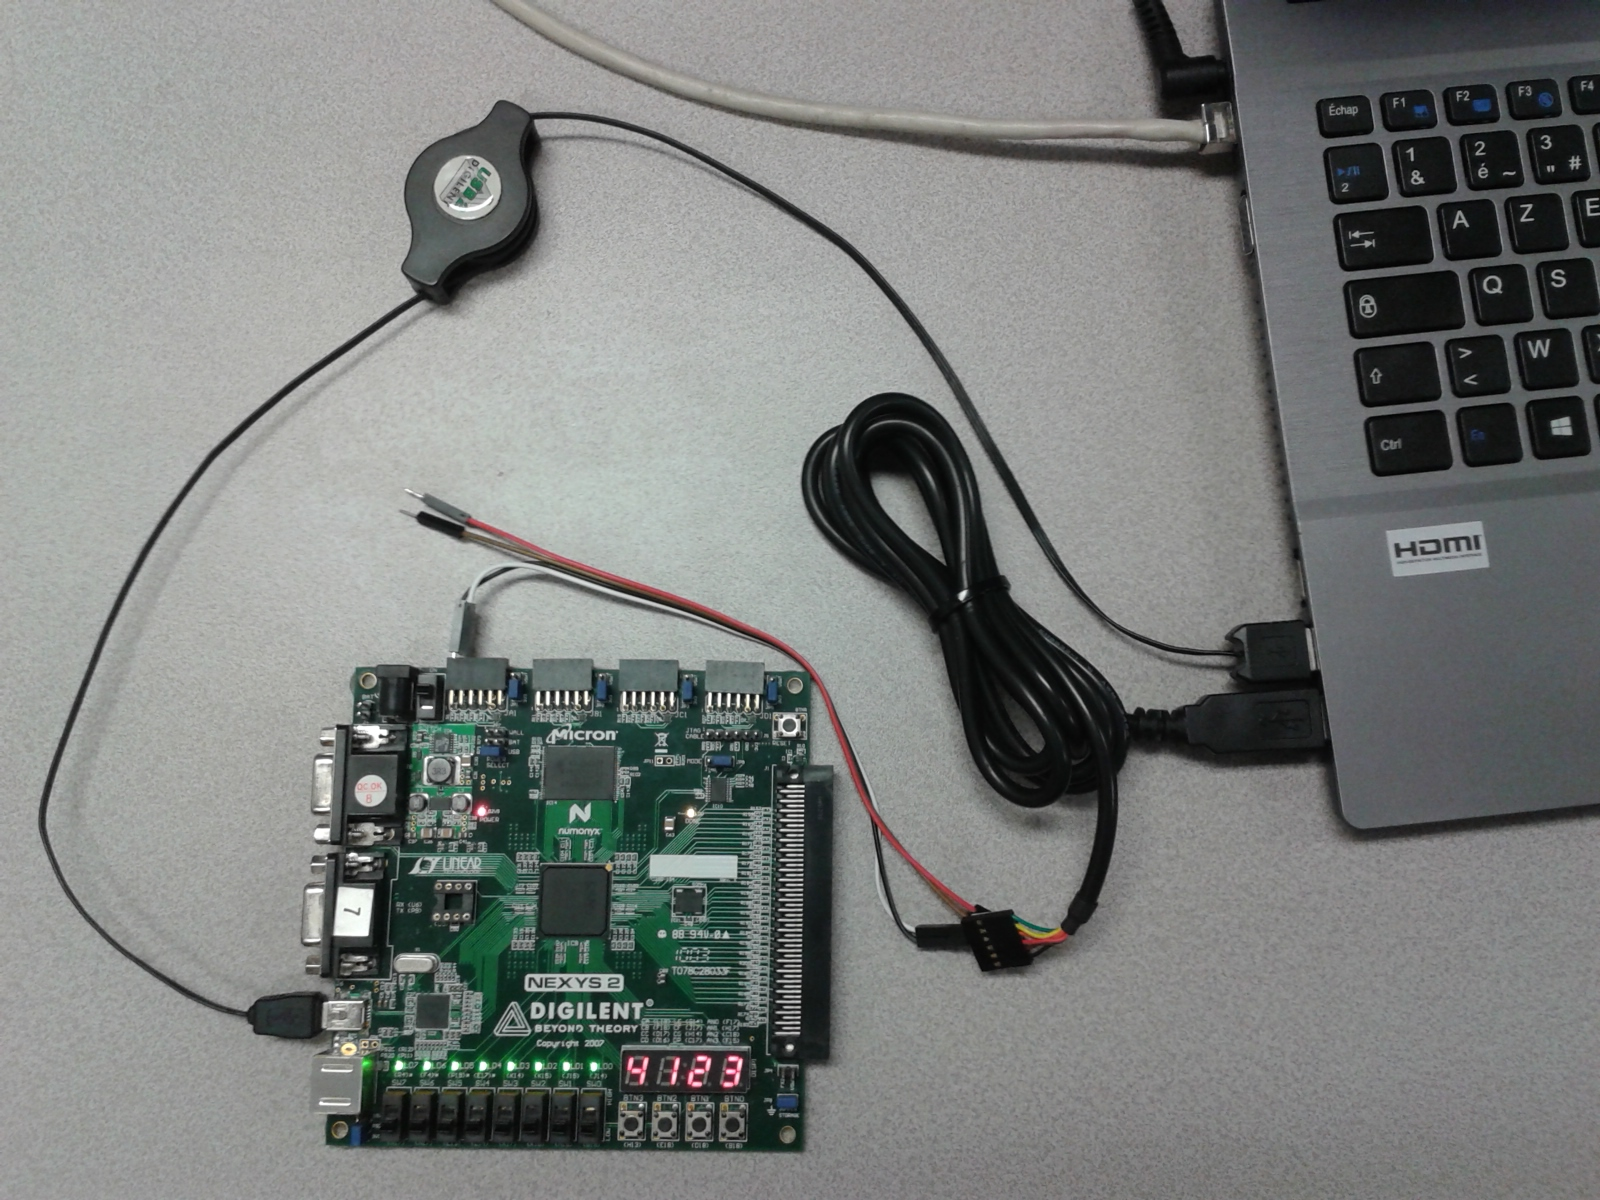
\includegraphics[width=\textwidth, keepaspectratio]{fig/Nexys2.jpg}
        \caption{A Nexys2 board}
      \end{figure}
    \end{frame}

  \section{Project management}

    \subsection{Risks}

    \begin{frame}
      We were able to identify real risks, and mitigate them.
    \end{frame}

    \subsection{Specification}

    \subsection{Calendar}

  \section{Processor Changes}
    \begin{landscape}
        \begin{frame}
            \includegraphics[scale=0.22]
                            {build/micromachine_updated_fromsvg.pdf}

        \end{frame}
    \end{landscape}
  \section{Implementation}

    \subsection{Compiler}

    \begin{frame}
      \begin{itemize}
        \item Based on the compiler project from the second-year classes.
        \item Language: a (quite large!) subset of C.
        \item Various optimizations.
      \end{itemize}
    \end{frame}

    \subsection{Interrupts}

    \begin{frame}
      \begin{itemize}
        \item Processor modifications.
        \item Priority support.
        \item Interrupt table.
      \end{itemize}
    \end{frame}

    \subsection{Scheduler}

    \begin{frame}
      \begin{itemize}
        \item New interrupt based on the PWM...
        \item that will trigger a context switch.
      \end{itemize}
    \end{frame}

    \subsection{Serial Port}

    \begin{frame}
      \begin{itemize}
        \item New interrupt.
        \item Limitations.
      \end{itemize}
    \end{frame}

    \subsection{Memory Management}
    
    \begin{frame}
      \begin{itemize}
        \item dynamic allocation
        \item malloc, free, realloc
        \item very simple implementation
        \item we keep the PID in the block headers
      \end{itemize}
    \end{frame}

    \subsection{Dynamic loading}
 
    \begin{frame}
      \begin{itemize}
        \item Not very hard to do...
        \item ...but we had to make the code position-independent.
      \end{itemize}
    \end{frame}

  \section{Final result}
 
  \begin{frame}{Various processes}
      \begin{itemize}
        \item The shell (most important)
        \item Counter
        \item Leds
        \item ... and dynamic loading !
      \end{itemize}
  \end{frame}

  \begin{frame}{Demo}
    \begin{itemize}
      \item Compiler
      \item Debugger
      \item Serial console
      \item Process management
    \end{itemize}
  \end{frame}

  \section{Use / improvements}

  \begin{frame}{Pedagogic use}
      Use in classes? Pedagogic interest.
  \end{frame}

\end{document}
